\documentclass[11pt]{ctexart}

\usepackage{multicol}
%\usepackage{mwe}
\usepackage{subfigure}
\usepackage{mathtools}
\usepackage{graphicx}
\usepackage{amsmath}
\usepackage{mathrsfs}
\usepackage[top=0.5in,bottom=1in,left=1in,right=1in]{geometry}
\usepackage{pdflscape}
\usepackage{times}
\usepackage{bm}
%\usepackage{setspace}
\usepackage{color}
\usepackage{caption}
\usepackage{amsmath}
\usepackage{amssymb}
\usepackage{CJK}
\usepackage{longtable}
%\usepackage[final]{pdfpages}
\usepackage{listings}
\usepackage{textcomp}
\usepackage{xcolor}
\usepackage{algorithm2e}
\usepackage{float}
\usepackage{algorithmicx}
\usepackage{algpseudocode}
\usepackage{hyperref}

\hypersetup{hidelinks,
	colorlinks=true,
	allcolors=black,
	pdfstartview=Fit,
	breaklinks=true}

\pagestyle{plain}




\begin{document}

\title{第十六周实习报告20220704}
\author{宋欣源}
\date{\today}

\maketitle % need full-width title

\CTEXsetup[format={\Large\bfseries}]{section}

\section{第一,综述}

下面对于这些天实习的工作做一个报告。现在就这一周的工作做一个总结
我这周主要在raw3数据集上进行。首先是研究了激活函数和初始化条件用于提高模型的稳定性,接下来研究原来backbone的模型并进行筛选,最后研究resnet模型并且进行调试。由于我的主要工作是基于raw3数据集,所以这篇报告暂时没有用到raw4数据集。最高达到pnl=2.99

\section{第二,稳定性研究}

\subsection{激活函数}
首先进行了稳定性研究,在激活函数和初始化上进行了模型改造,选取以前表现最好的三个模型作为基础,做了大量实验。首先,对于不同的激活函数,有如下几种:
\begin{itemize}
  \item [0)]
    nn.relu常用激活函数,效果是能让模型快速收敛,但是不宜太多,
  \item [1)]
    nn.LeakyReLU,relu的魔改版本,效果不好,收敛速度慢,直接抛弃
  \item [2)]
    nn.sigmoid 经过大量实验,效果不好,不再使用,影响原来模型的效果
  \item [3)]
    nn.softmax 只适用于某一维度数据,有少量提升,进行试验如下
  \item [4)]
    nn.tanh 效果和relu一样,但是收敛速度很慢,不适合大量实验

\end{itemize}

baseline:普通CNN1d((CNN1d(5,1)+batchnorm)*3+relu+CNN1d(3,1)+

dropout+batchnorm+relu+

CNN1d(3,1)+CNN1d(3,1)+CNN1d(3,1)+batchnorm+relu+avg+dropout+

CNN1d(3,1)+CNN1d(3,1)+CNN1d(3,1)+batchnorm+dropout+avg+avg+linear)

模型表现{\kaishu \small IC: 0.069, pnl:2.783}

~\\
模型1:普通CNN1d((CNN1d(5,1)+batchnorm)*3+softmax+relu+CNN1d(3,1)+

dropout+batchnorm+softmax+relu+

CNN1d(3,1)+CNN1d(3,1)+CNN1d(3,1)+batchnorm+softmax+relu+avg+dropout+

CNN1d(3,1)+CNN1d(3,1)+CNN1d(3,1)+batchnorm+dropout+avg+avg+softmax+linear)

softmax激活函数的意义是换成概率分布。因此在特定的地方不能出现,否则模型无法学习。首先将relu都换成softmax,效果不好,快速下降的目的没有起到,出现梯度消失,稳定性也不好。因此采用了relu+softmax。最后效果略有下降,但是稳定性大幅提高。尝试batchnorm去掉,不如这种效果好。

模型表现{\kaishu \small IC: 0.068, pnl:2.691}

~\\
模型2:普通CNN1d((CNN1d(5,1)+batchnorm)*3+softmax+relu+CNN1d(3,1)+

dropout+batchnorm+relu+

CNN1d(3,1)+CNN1d(3,1)+CNN1d(3,1)+batchnorm+relu+avg+dropout+

CNN1d(3,1)+CNN1d(3,1)+CNN1d(3,1)+batchnorm+dropout+avg+avg+softmax+linear)

进行大量尝试后,在开头和结尾加入softmax,结果有提高,稳定性也能一次跑通.在此基础上进行了大量实验,稳定性有提高,但是表现上不去。在另外两个baseline上也是同样结果。

模型表现{\kaishu \small IC: 0.070, pnl:2.727}

\subsection{初始化条件}
cnn会对模型进行初始化,不需要特别关注,但是对于不同模型,初始化要求不一样,原来模型的初始化可能错过表现极值点,常识的初始化条件有这几种:
\begin{itemize}
  \item [0)]
    torch.nn.init.uniform\_(tensor, a=0, b=1)均匀分布初始化,稳定性较差,比原来不好
  \item [1)]
    torch.nn.init.normal\_(tensor, mean=0.0, std=1.0)正态(高斯)分布初始化,稳定性很好,但是影响最后表现。原因可能与数据较稳定,不利于找到最后结果有关。以后不再采用normal初始化
  \item [2)]
    torch.nn.init.xavier\_uniform\_(tensor, gain=1.0)和torch.nn.init.xavier\_normal\_(tensor, gain=1.0)值适用于二维数据初始化,但是目前情况不方便支队二维初始化。
  \item [3)]
    torch.nn.init.orthogonal\_(tensor, gain=1)正交初始化,由于超出的维度就会被flartten化,容易造成梯度消失,torch.nn.init.sparse\_(tensor, sparsity, std=0.01)容易造成梯度消失,\par torch.nn.init.constant\_(tensor, val),容易造成梯度消失。从这一点来看,rnn之前设置的初始条件不很理想,应该用别的办法初始化hidden\_state。torch.nn.init.eye\_(tensor)单位矩阵初始化,只适用于两维矩阵,\par torch.nn.init.zeros\_(tensor)零填充初始化,容易造成梯度消失,weight=0.
  \item [4)]
    最有用的就是kaiming\_normal和kaiming\_uniform初始化,特点在于,维持权值的方差,在训练和推理的时候,维持方差不变。维持方差不变的好处是,在传播和反向传播的时候,不会造成整个矩阵的参数偏离。这个初始化方法只使用于relu和LeakyReLU激活函数,因此,对于三种baseline model都进行了尝试。需要注意的是,kaiming\_normal和kaiming\_uniform都仅限3维度以上的模型,因此最后的linear层都不初始化,所有的cnn层加上bias=False。

\end{itemize}

baseline:普通CNN1d((CNN1d(5,1)+batchnorm)*3+softmax+relu+CNN1d(3,1)+

dropout+batchnorm+relu+

CNN1d(3,1)+CNN1d(3,1)+CNN1d(3,1)+batchnorm+relu+avg+dropout+

CNN1d(3,1)+CNN1d(3,1)+CNN1d(3,1)+batchnorm+dropout+avg+avg+softmax+linear)

模型表现{\kaishu \small IC: 0.065, pnl:2.765}

~\\
模型1:CNN1d((CNN1d(5,1)+batchnorm)*3+softmax+relu+CNN1d(3,1)+

dropout+batchnorm+softmax+relu+

CNN1d(3,1)+CNN1d(3,1)+CNN1d(3,1)+batchnorm+softmax+relu+avg+dropout+

CNN1d(3,1)+CNN1d(3,1)+CNN1d(3,1)+batchnorm+dropout+avg+avg+linear+softmax)

kaiming\_normal初始化,a = 0,mode = 'fan\_in',nonlinearity='relu'

模型稳定性大大提高,表现也有提高,以后采用这个初始化。

模型表现{\kaishu \small IC: 0.071, pnl:2.792}

~\\
模型2:CNN1d((CNN1d(5,1)+batchnorm)*3+softmax+relu+CNN1d(3,1)+

dropout+batchnorm+softmax+relu+

CNN1d(3,1)+CNN1d(3,1)+CNN1d(3,1)+batchnorm+softmax+relu+avg+dropout+

CNN1d(3,1)+CNN1d(3,1)+CNN1d(3,1)+batchnorm+dropout+avg+avg+linear+softmax)

kaiming\_uniform初始化,a = 0,mode = 'fan\_in',nonlinearity='relu'

和uniform有关,模型稳定性很高,但是模型表现大幅下降。以后不再使用
模型表现{\kaishu \small IC: 0.054, pnl:2.355}

\subsection{总结}

在稳定性上经过了大量实验,找到了最适合的激活函数和最适合的初始化办法。以后按这个方法来做。但是,目前模型参数较少,backbone解释力有限,同时深度太高也不能解决问题,尝试采用背的backbone重新搭建模型。


\section{第三,CNN1d-old}
\subsection{综述}
在原有CNN1d上进行了大量实验。现在结果明显变好,将原来模型深度从10层提高到15层cnn1d并且进行细节的调整。基于上一周的经验,模型需要有更好的稳定性,能持续在某个范围坚持。不能过快的过拟合。基于上一周的经验,发现尺缩模型结果更好,尺度缩窄以后,减少了linear,pointwise等层的作用,导致模型参数更多的在卷积层上进行梯度下降和拟合。然而,尺度缩窄以后,后面的模型提取的信息具有更大的不确定性,不能很好的表现所有数据的特性,那么还是采取最后加入avgpool的方式提高模型在时间序列的表现。

\subsection{模型和表现}

模型1:普通CNN1d(CNN1d(5,1)*3+relu+batchnorm+CNN1d(3,1)+

CNN1d(1,1)*2+batchnorm+relu+linear)

模型表现{\kaishu \small IC: 0.054, pnl:2.52}

~\\
模型2:普通CNN1d(CNN1d(5,1)*3+relu+batchnorm+CNN1d(3,1)+

CNN1d(1,1)*2+batchnorm+relu+pointwise*3)

模型表现{\kaishu \small IC: 0.061, pnl:2.563}

这个模型加入dropout后表现有所提升,梯度下降变慢

模型表现{\kaishu \small IC: 0.062, pnl:2.607}

~\\
模型3:普通CNN1d(CNN1d(5,1,256)*3+relu+batchnorm+CNN1d(3,1,512)+

CNN1d(1,1,512)*2+batchnorm+relu+linear)

将hidden\_channel提高,模型过拟合速度变快,但是并没有效果变好

模型表现{\kaishu \small IC: 0.057, pnl:2.564}

~\\
模型4:普通CNN1d(CNN1d(5,1)*3batchnorm+relu+avg+CNN1d(3,1)

+cnn1d(1,1)*2+batchnorm+relu+avgpool+cnn1d(3,1)

+cnn1d(1,1)*2+batchnorm+relu+avgpool+cnn1d(3,1)

+CNN1d(1,1)*2+relu+dropout+linear)

将模型的卷积层数提高到15层,注意顺序一定是cnn1d+batchnorm+relu+avgpool

三个模块的组合,这种方式经过大量实验是效果最好的,pnl普遍在2.7以上,下面就进行微调,首先肯定是在尺缩上下文章。卷积核的设置是种类越多越好,尺缩相反,经过大量实验,只采取两种池化长度的尺缩模型效果最好。所以采用avgpool(3,3)和avgpool(5,5)进行操作,进一步提高效果。

模型表现{\kaishu \small IC: 0.069, pnl:2.788}

~\\
模型5:普通CNN1d(CNN1d(5,1)*3batchnorm+relu+avg(5,5)+CNN1d(3,1)

+cnn1d(1,1)*2+batchnorm+relu+avgpool(3,3)+cnn1d(3,1)

+cnn1d(1,1)*2+batchnorm+relu+avgpool(3,3)+cnn1d(3,1)

+CNN1d(1,1)*2+relu+dropout+linear)

采用5池化长度和3池化长度的avgpool,放在合适的位置上

模型表现{\kaishu \small IC: 0.071, pnl:2.801}

~\\
模型6:普通CNN1d(CNN1d(5,1)*3batchnorm+relu+avg(5,1)+CNN1d(3,1)

+cnn1d(1,1)*2+batchnorm+relu+avgpool(3,3)+cnn1d(3,1)

+cnn1d(1,1)*2+batchnorm+relu+avgpool(3,3)+cnn1d(3,1)

+CNN1d(1,1)*2+batchnorm+relu+avgpool(3,3)+dropout+linear)

池化5长度不产生尺缩,3长度产生尺缩,这样做,结果是模型的训练具有偏好,池化长度为5之前的参数几乎训练不动,但是效果又稍微提高,不采取这个模式,因此stride还是都设置为和kernel\_size一样。

模型表现{\kaishu \small IC: 0.071, pnl:2.850}

~\\
模型7:普通CNN1d(CNN1d(5,1)*3batchnorm+relu+avg(5,5)+CNN1d(3,1)

+cnn1d(1,1)*2+batchnorm+relu+avgpool(3,1)+cnn1d(3,1)

+cnn1d(1,1)*2+batchnorm+relu+avgpool(3,1)+cnn1d(3,1)

+CNN1d(1,1)*2+batchnorm+relu+avgpool(3,3)+dropout+linear)

对于3和5的各种组合都进行了尝试,最好的结果就是这个模型,没有模型8的只采用3效果好。模型4-8是这个backbone下的五个尺缩版本。

模型表现{\kaishu \small IC: 0.071, pnl:2.865}


~\\
模型8:普通CNN1d(CNN1d(5,1)*3batchnorm+relu+avg(3,3)+CNN1d(3,1)

+cnn1d(1,1)*2+batchnorm+relu+avgpool(3,3)+cnn1d(3,1)

+cnn1d(1,1)*2+batchnorm+relu+avgpool(3,3)+cnn1d(3,1)

+CNN1d(1,1)*2+batchnorm+relu+avgpool(3,3)+dropout+linear)

经过大量实验,模型8是表现最好的模型,只采用kernel\_size和stride一样的3池化长度,得到了目前最好的结果。而且模型在2.7以上能坚持5个epoche。经过weight check发现模型参数都在变化,没有出现参数训练不动的情况。这个模型接下来还有挖掘空间。

模型表现{\kaishu \small IC: 0.078, pnl:2.93}

表现如下:
\begin{figure}[H]

\begin{center}
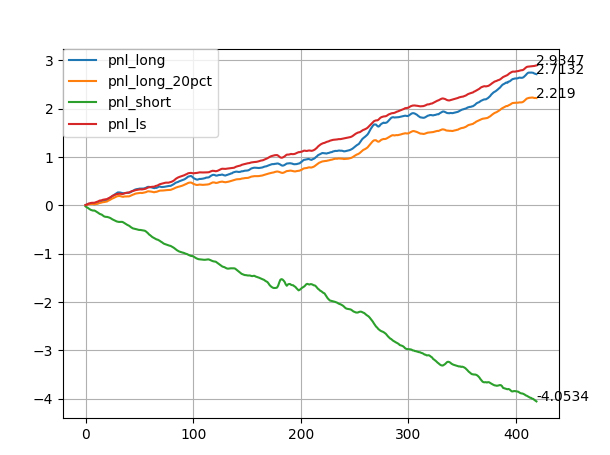
\includegraphics[width=0.8\textwidth]{1.PNG}
\end{center}
\caption{CNN1d pnl fugure}
\label{FIG.1}
\end{figure}

~\\
模型9:普通CNN1d(CNN1d(5,1)*3batchnorm+relu+avg(3,3)+CNN1d(3,1)

+(cnn1d(1,1)*2+batchnorm+relu+avgpool(3,3)+cnn1d(3,1))*3

+CNN1d(1,1)*2+batchnorm+relu+avgpool(3,3)+dropout+linear)

将模型的深度大大提高,提高到30层这时候模型有所失效,经过实验发现层数提高,从15提高到50的过程中,效果越来越差,无论是在拟合还是过拟合上都有所欠缺。很容易想到是深度增加,但是数据量有限的情况下模型整体偏移的结果。因此开始采用resnet进行训练,将每两层加入resnet结构。

模型表现{\kaishu \small IC: 0.078, pnl:2.58}

\iffalse  %
\section{第四,resnet50}
\subsection{综述}
resnet的结构就是residual,有多种结构,如下图:
\begin{figure}[H]

\begin{center}
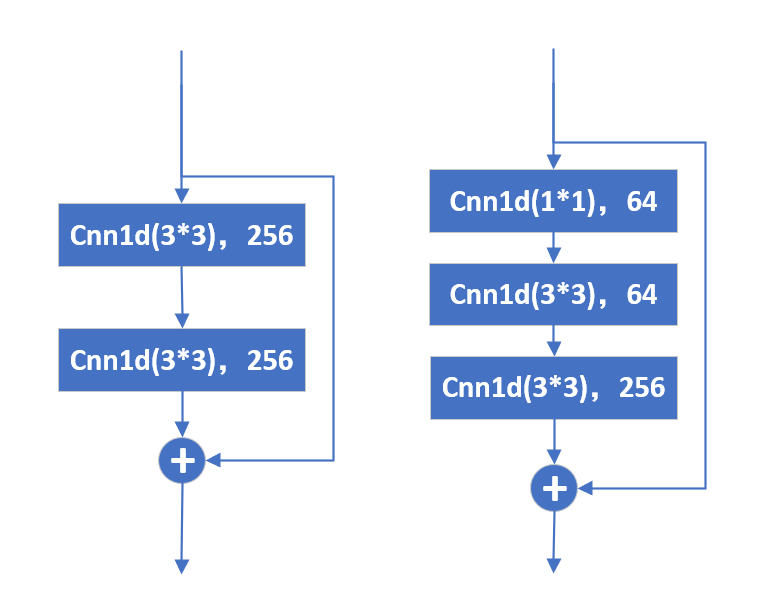
\includegraphics[width=0.8\textwidth]{residual1.PNG}
\end{center}
\caption{residual structure}
\label{FIG.2}
\end{figure}

按照这两种结构进行堆叠,成如下的结构,把这种结构在上面的30层cnn1d上进行应用,如图:
\begin{figure}[H]

\begin{center}
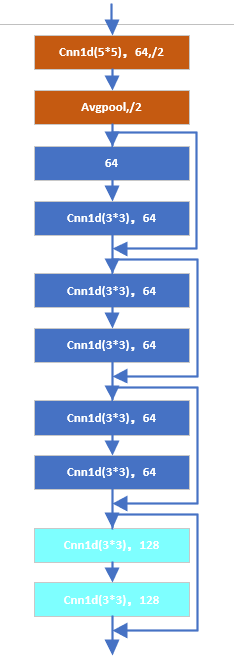
\includegraphics[width=0.8\textwidth]{residual3.PNG}
\end{center}
\caption{residual cnn1d30 structure}
\label{FIG.3}
\end{figure}

加入了residual,具体的细节结构还需要进一步尝试,究竟shortcut是插入在avg之中,relu之中还是batchnorm以后。以及resnet50的residual结构都在上面的30层cnn1d上进行应用。得到如下的的模型。

除了这两种结构以外,还可以对residual的结构进行调整,

~\\
模型1:Resnet3(256)

这个模型是3层resnet,hidden\_size是256的模型,采用了两种

模型表现{\kaishu \small IC: 0.068, pnl:2.720}

~\\
模型10:普通CNN1d((CNN1d(5,1)+batchnorm)*3+relu+CNN1d(3,1)+batchnorm+relu+

CNN1d(3,1)+CNN1d(3,1)+CNN1d(3,1)+batchnorm+relu+avg

CNN1d(3,1)+CNN1d(3,1)+CNN1d(3,1)+batchnorm+dropout+avg+avg+linear)

下面是提高模型深度,不妨让卷积再增加三层,卷积层增加以后,拟合效果变好,但是最后效果并没有提高。采用的办法是每三层记一次relu和avgpool

模型表现{\kaishu \small IC: 0.066, pnl:2.751}

~\\
模型11:普通CNN1d((CNN1d(5,1)+batchnorm)*3+relu+CNN1d(3,1)+

dropout+batchnorm+relu+

CNN1d(3,1)+CNN1d(3,1)+CNN1d(3,1)+batchnorm+relu+avg+dropout+

CNN1d(3,1)+CNN1d(3,1)+CNN1d(3,1)+batchnorm+dropout+avg+avg+linear)

为了降低过拟合,在三个模块中间都加入了dropout,果然训练变得缓慢下降,效果也有小幅提高。稳定性有所降低.

模型表现{\kaishu \small IC: 0.069, pnl:2.783}

表现如下:
\begin{figure}[H]

\begin{center}
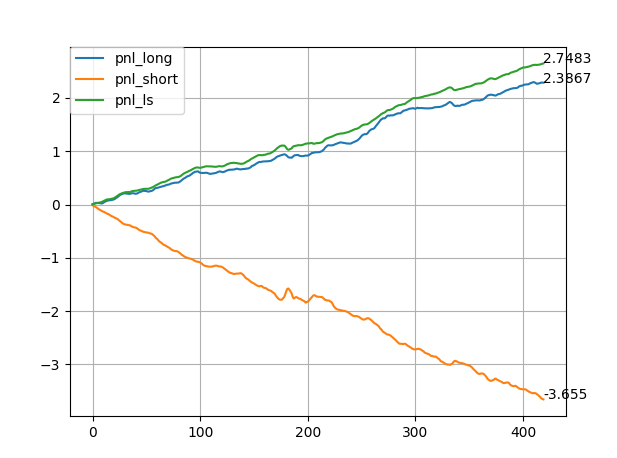
\includegraphics[width=0.8\textwidth]{2.PNG}
\end{center}
\caption{CNN1d pnl fugure}
\label{FIG.1}
\end{figure}

经过上面的研究,取得了不错的效果,但是效果还不够。因此又做了大量尝试,结果都差不多。直接想到应该继续加深模型,有了以下这些模型结果

~\\
模型12:普通CNN1d((CNN1d(5,1)+batchnorm)*3+relu+CNN1d(3,1)+

dropout+batchnorm+relu+

CNN1d(3,1)+CNN1d(3,1)+CNN1d(3,1)+batchnorm+relu+avg+dropout+

CNN1d(3,1)+CNN1d(3,1)+CNN1d(3,1)+batchnorm+relu+avg+dropout+

CNN1d(3,1)+CNN1d(3,1)+CNN1d(3,1)+batchnorm+dropout+avg+avg+linear)

模型深度提高,效果提高,骨架结构还是采用的之前研究的结构,兼顾稳定性和效果。

模型表现{\kaishu \small IC: 0.072, pnl:2.821}

~\\
模型13:普通CNN1d((CNN1d(5,1)+batchnorm)*3+relu+CNN1d(3,1)+

dropout+batchnorm+relu+

CNN1d(3,1)+CNN1d(3,1)+CNN1d(3,1)+batchnorm+relu+avg+dropout+

CNN1d(1,1)+CNN1d(1,1)+CNN1d(1,1)+batchnorm+dropout+avg+avg+linear)

不妨想到,cnn的格式可以不拘于一格,也体现出跨步跳跃的情况。不妨采用kernel\_size = 1的卷积层作为最后三层,经过大量实验,效果超过了同层的三卷积层。从理解上,应该是类似\par bottleneck结构。在高维卷积后面加入1维卷积效果会有提升。

模型表现{\kaishu \small IC: 0.075, pnl:2.830}

~\\
模型14:普通CNN1d((CNN1d(5,1)+batchnorm)*3+relu+CNN1d(3,1)+

dropout+batchnorm+relu+

CNN1d(3,1)+CNN1d(3,1)+CNN1d(3,1)+batchnorm+relu+avg+dropout+

CNN1d(1,1)+relu+CNN1d(1,1)+relu+CNN1d(1,1)+batchnorm+dropout+avg+avg+linear)

继续跳跃,在每个1卷积层后加入relu.

模型表现{\kaishu \small IC: 0.074, pnl:2.789}

~\\
模型15:普通CNN1d((CNN1d(5,1)+batchnorm)*3+relu+CNN1d(3,1)+

dropout+batchnorm+relu+

CNN1d(3,1)+CNN1d(3,1)+CNN1d(3,1)+batchnorm+relu+avg+dropout+

CNN1d(3,1)+CNN1d(3,1)+CNN1d(3,1)+batchnorm+relu+avg+dropout+

CNN1d(1,1)+relu+CNN1d(1,1)+relu+CNN1d(1,1)+batchnorm+dropout+avg+avg+linear)

模型深度继续增加,发现效果变差。经过实验,CNN的层数不适合超过9层,因此,对于\par CNN1d的模型首先必须要确定模型能承受的CNN层数上限。对于以后的模型设计有很大帮助。

模型表现{\kaishu \small IC: 0.055, pnl:2.520}

~\\
模型15:普通CNN1d((CNN1d(5,1)+batchnorm)*3+relu+CNN1d(3,1)+

dropout+batchnorm+relu+

CNN1d(1,1)+CNN1d(3,1)+batchnorm+relu+avg+dropout+

CNN1d(1,1)+relu+CNN1d(1,1)+relu+CNN1d(1,1)+batchnorm+dropout+avg+avg+linear)

模型结构进行大的修改,发现还有实验的新天地。也就是不同kernel\_size的组合。经过之前模型的实验已经知道,尽可能多种类的kernel\_size的效果更好,但是稳定度较差。那么思路应该是尽可能尝试不同的kernel\_size的组合。对于稳定性,采用其他层加以巩固。

模型表现{\kaishu \small IC: 0.065, pnl:2.758}

表现如下:
\begin{figure}[H]

\begin{center}
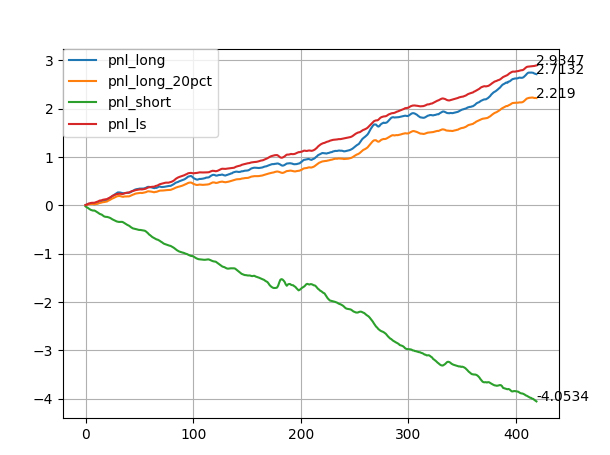
\includegraphics[width=0.8\textwidth]{1.PNG}
\end{center}
\caption{CNN1d pnl fugure}
\label{FIG.2}
\end{figure}

\subsection{改进思路}
\begin{itemize}
  \item [0)]

  \item [1)]

  \item [2)]

\end{itemize}


\section{第四,transformer的感悟和回炉}
\fi %

\section{第五、总结}
\begin{itemize}
  \item [1)]
  这一周半,从模型稳定性和新的backbone出发,主要是进行了大量实验,自己又研究出一批CNN1d模型,同时会在这些模型上深入。从dialtion,groups,stride上下功夫,\par 同时在不同kernel\_size的组合上下功夫。
  \item [2)]
  第二,对于模型稳定性,找到了最适合的激活函数和特定的表达方式,积累了大量经验。对于初始化,以后采用kaiming\_normal的初始化方式。
  \item [3)]
  第三,对于CNN1d系列,下周就继续搭建自己新的backbone。
  \item [4)]
  第四,对于transformer模型,这周有了很深的启发,找到了以前模型没学到东西的原因。下周开始进一步训练。
\end{itemize}


\end{document} 